\section{Mulvariate Binary Regression}
Also known as \textit{logistic regression}. The activation is:
\[
  \hat{a}(\vec{x})= \frac{1}{1+e^{-(\vec{w}\cdot{}\vec{x}+b)}}
\]

plot for 1 feature on figure \ref{fig:sigmoid}. By tuning $w$ and $b$  we can find the best fit. 

The sign of $w$ reflects the line over $y$ axis, the magnitude controls the slope. Again, $b$ translates over $x$.

\begin{figure}[h]
 \centering
 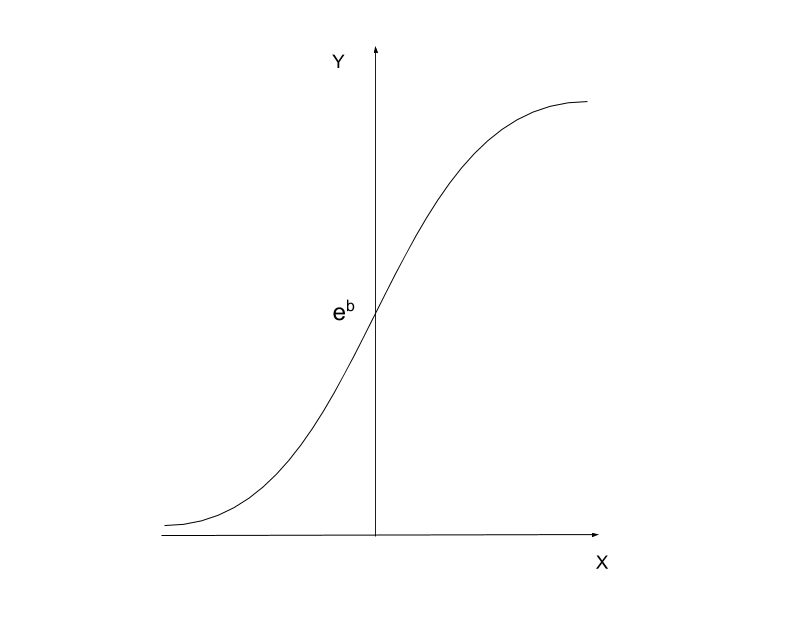
\includegraphics[width=0.9\textwidth]{sigmoid_plot.png}
  \caption{Sigmoid. Mistake: at $x=0$, $y=(e^{-b}+1)^{-1}$} \label{fig:sigmoid}
\end{figure}

\subsection{Forward Propagation}
The network schema can be found in \ref{fig:single}. It is used to build the calculations:

\begin{itemize}
  \item The activation is a \textit{sigmoid} function:
\[
  \hat{a}_i = \frac{1}{1+e^{-(\sum_j w_j\, \mathbf{X}_{ji} + b)}}
\]

  \item The Loss is the Cross Entropy Loss:
\[
  L_i = a_i\,\log(\hat{a}_i) + (1-a_i)\,\log(1-\hat{a}_i)
\]

\item The cost:
\[
  C(\vec{w}, b) = -\frac{1}{m}\sum_{i=0}^m L_i(\vec{w}, b)
\]
\end{itemize}
This is coded:
\begin{verbatim}
cost = 1/m*(np.dot(A, np.log(Ap).T) 
+ np.dot(1-A, np.log(1-Ap).T))
#or
Cost = 1/m*(np.sum(np.multiply(A, np.log(Ap)) 
+ np.multiply(1-A, np.log(1-Ap))))
#tested
\end{verbatim}

\subsection{Backward propagation}

\begin{align}
  \frac{\partial L_i}{\partial w_j} = 
  \left(\frac{\partial L_i}{\partial \hat{a}_i}\, \frac{\partial \hat{a}_i}{\partial z_i}\right)\,\frac{\partial z_i}{\partial w_j}\\
  \frac{\partial L_i}{\partial b} = 
  \left(\frac{\partial L_i}{\partial \hat{a}_i}\,\frac{\partial \hat{a}_i}{\partial z_i}\right)\,\frac{\partial z_i}{\partial b}
\end{align}
The first two derivatives (enclosed in parens) are the same, let's compute them.

\begin{align*}
  \frac{\partial L_i}{\partial \hat{a}_i} &= \frac{a_i}{\hat{a}_i} + \frac{(1-a_i)}{1-\hat{a}_i}\,(-1) \\
%  \frac{\partial \hat{a}_i}{\partial z_i} &= \ldots  \label{eq:derZ}\\
%  a(z)&= \frac{1}{1+e^{-z}}\\ we can apply parts if we want
%  a(u)&=\frac{1}{u}\\
%  da&=-u^{-2}\,du\\
  \frac{d\hat{a}_i}{dz_i}&=-\left(\frac{1}{1+e^{-z}}\right)^{-2}\,e^{-z}(-1)\\
  &=\left(\frac{1}{1+e^{-z}}\right)^{-2}\,(e^{-z} + 1 -1)\\
  &= \hat{a}^2\,(\frac{1}{\hat{a}} -1) \\
  \frac{\partial \hat{a}_i}{\partial z_i} &= \hat{a}_i\,(1-\hat{a}_i)
\end{align*}
Hence the derivative is:
\begin{align*}
  \frac{\partial L_i}{\partial \hat{a}_i}\,\frac{\partial \hat{a}_i}{\partial z_i} &= \left[ \frac{a_i}{\hat{a}_i} + \frac{(1-a_i)}{1-\hat{a}_i}\,(-1) \right]\,\hat{a}_i\,(1-\hat{a}_i)\\
  &= a_i - \hat{a}_i\\
  \frac{\partial z_i}{\partial w_j} &= \mathbf{X}_{ji}\\
  \frac{\partial z_i}{\partial b} &= 1
\end{align*}
We are left with:

\begin{align*}
  \frac{\partial L_i}{\partial \hat{a}_i}\,\frac{\partial \hat{a}_i}{\partial z_i}\,\frac{\partial z_i}{\partial w_j} &= \left(a_i - \hat{a}_i\right)\,\mathbf{X}_{ji}\\
  \frac{\partial L_i}{\partial \hat{a}_i}\,\frac{\partial \hat{a}_i}{\partial z_i}\,\frac{\partial z_i}{\partial b} &= \left(a_i - \hat{a}_i\right)\,1\\
\end{align*}

We then have:
\begin{align*}
  w_j &= w_j - \alpha\frac{\partial C}{\partial w_j}\\
  &= w_j + \frac{\alpha}{m}\sum \frac{\partial L_i}{\partial w_j}\label{eq:same}\\
  &= w_j + \frac{\alpha}{m}\sum_i (a_i-\hat{a}_i)\mathbf{X}_{ji}
\end{align*}
But we can compute in general:
\begin{align}
  \vec{w} &= \vec{w} - \frac{\alpha}{m}\,\frac{\partial C}{\partial \vec{w}}\nonumber\\
  &= \vec{w} + \frac{\alpha}{m}\,\mathbf{X}\cdot{}\mathbf{\Delta A}^T\\
  b &= b - \frac{\alpha}{m}\,\frac{\partial C}{\partial b}\nonumber\\
  &= b + \frac{\alpha}{m}\mathbf{\Delta A}
\end{align}

The same result than for linear regression. 
